\documentclass[Orbiter Technical Reference.tex]{subfiles}
\begin{document}

\section{Dynamic state vector propagation}
\textbf{Martin Schweiger}\\
\textbf{September 28, 2017}


\subsection{Introduction}
This document describes the numerical integration methods used by Orbiter to propagate vessel state vectors from one time point to the next. The time step intervals can vary over a large range, both due to variations in the computational complexity of rendering a frame for the 3D scenery, and due to support for ``time compression'' up to $10^5 \times$ real time.
To avoid the accumulation of numerical errors during the simulation, integration schemes of adequate accuracy must be chosen.
Where the time intervals become too large to allow sufficiently accurate numerical integration of the state vectors, Orbiter can switch to ``orbit stabilisation'', a variant of \emph{Encke's method}, where only the perturbations on top of a base line 2-body orbit defined by its osculating elements are integrated numerically.

\subsection{Polynomial interpolation methods}
Let $\vec{r}_n$ and $\vec{v}_n$ be the state vectors of a vessel at time $t_n$, given in some coordinate system. Let the interval to the next step $t_{n+1}$ be given by $\Delta t_n = t_{n+1}-t_n$.
 In the following, we assume that the gravitational acceleration $\vec{a}_g$ at any position $\vec{r}$ and any time $t$ between $t_n$ and $t_{n+1}$ can be computed. Further we assume that any additional forces $\vec{a}_0$ (thrust, atmospheric drag, etc.) are constant between $t_n$ and $t_{n+1}$.
\begin{equation*}
\vec{a}(t) = \vec{a}_g(t,\vec{r}(t)) + \vec{a}_0 \equiv \ACC(t,\vec{r}),\qquad t \in [t_n, t_{n+1}]
\end{equation*}
where operator $\ACC$ formally denotes the function call providing the forces acting on the vessel at an arbitrary time within $[t_n, t_{n+1}]$.
This will generally involve the summation of numerically calculated gravitational potentials from relevant celestial bodies.
The equation of motion is then given by the 2nd order differential equation
\begin{equation}\label{eq:motion}
\ddot{\vec{r}} = \ACC(t,\vec{r})
\end{equation}
The following sections describe methods used in the Orbiter code to solve the initial value problem of propagating $(\vec{r}_n,\vec{v}_n)$ to $(\vec{r}_{n+1},\vec{v}_{n+1})$.

\subsubsection{Linear interpolation, single pass [L/s]}
Given state vectors ($\vec{r}_n$, $\vec{v}_n$) and $\vec{a}_n = \ACC(t_n,\vec{r}_n)$, and interval $h=\Delta t_n$, calculate $(\vec{r}_{n+1},\vec{v}_{n+1})$ using a predictor-corrector method with a linear interpolation of $\vec{a}$.
Let
\begin{equation*}
\vec{r}_{n+1}^{(0)} = \vec{r}_n + h\vec{v}_n + \frac{1}{2} h^2\vec{a}_n
\end{equation*}
be the predicted new position under the assumption of constant $\vec{a}(t) = \vec{a}_n$. (Zero-th order approximation).
Recalculate the acceleration at the predicted position:
\begin{equation*}
\vec{a}_{n+1}^{(0)} = \ACC(t_{n+1},\vec{r}_{n+1}^{(0)})
\end{equation*}
Assume a linear interpolation of $\vec{a}$ between $t_n$ and $t_{n+1}$:
\begin{equation*}
\vec{a}(t) = \vec{a}_n + (\vec{a}_{n+1}^{(0)}-\vec{a}_n)\frac{t-t_n}{h},
\qquad t \in [t_n, t_{n+1}].
\end{equation*}
Then the state vector updates are given by
\begin{equation}
\begin{split}
\Delta\vec{v}^{(0)} &= \int_{t_n}^{t_{n+1}} \vec{a}(t) dt = \frac{1}{2}h (\vec{a}_n+\vec{a}_{n+1}^{(0)}) \\
\Delta\vec{r}^{(0)} &= \int_{t_n}^{t_{n+1}} \vec{v}(t) dt = \int_{t_n}^{t_{n+1}} \vec{v}_n + \vec{a}(t)t dt = h\vec{v}_n + \frac{1}{2}h\Delta\vec{v}^{(0)} \label{eq:lin_pos_upd}
\end{split}
\end{equation}
and thus
\begin{equation*}
\begin{split}
\vec{r}_{n+1} &= \vec{r}_n + \Delta\vec{r}^{(0)} \\
\vec{v}_{n+1} &= \vec{v}_n + \Delta\vec{v}^{(0)}
\end{split}
\end{equation*}

\subsubsection{Linear interpolation, double pass [L/d]}
The above method can be iterated further to provide a second correction. Given the position update of Eq.~\ref{eq:lin_pos_upd}, re-calculate the gravitational acceleration
\begin{equation*}
\vec{a}_{n+1}^{(1)} = \ACC(t_{n+1},\vec{r}_n+\Delta\vec{r}^{(0)})
\end{equation*}
and use the new acceleration estimate for the interpolation:
\begin{equation*}
\begin{split}
\Delta\vec{v}^{(1)} &= \frac{1}{2}h (\vec{a}_n+\vec{a}_{n+1}^{(1)}) \\
\Delta\vec{r}^{(1)} &= h\vec{v}_n + \frac{1}{2}h\Delta\vec{v}^{(1)}
\end{split}
\end{equation*}
and
\begin{equation*}
\begin{split}
\vec{r}_{n+1} &= \vec{r}_n + \Delta\vec{r}^{(1)} \\
\vec{v}_{n+1} &= \vec{v}_n + \Delta\vec{v}^{(1)}
\end{split}
\end{equation*}

\subsubsection{Quadratic interpolation, single pass [Q]}
To use a second-order interpolation of $\vec{a}(t)$ between $t_n$ and $t_{n+1}$, we first propagate the position by a half-step,
\begin{equation*}
\vec{r}_{n+\frac{1}{2}}^{(0)} = \vec{r}_n + \frac{h}{2} \vec{v}_n + \frac{1}{2}\left(\frac{h}{2}\right)^2\vec{a}_n
\end{equation*}
and find the mid-point acceleration,
\begin{equation}
\vec{a}_{n+\frac{1}{2}}^{(0)} = \ACC\left(t_n+\frac{h}{2},\vec{r}_{n+\frac{1}{2}}^{(0)}\right)\label{eq:acc_quad_half}
\end{equation}
which is then used to propagate across the full step,
\begin{equation*}
\vec{r}_{n+1}^{(0)} = \vec{r}_n + h\vec{v}_k + \frac{1}{2}h^2\vec{a}_{n+\frac{1}{2}}^{(0)}
\end{equation*}
and
\begin{equation}
\vec{a}_{n+1}^{(0)} = \ACC(t_{n+1},\vec{r}_{n+1}^{(0)})\label{eq:acc_quad_full}
\end{equation}
We now assume a quadratic behaviour of $\vec{a}(t)$ between $t_n$ and $t_{n+1}$:
\begin{equation*}
\vec{a}(t) = \vec{a}_n + \vec{c}_1 (t-t_n) + \vec{c}_2 (t-t_n)^2
\qquad t \in [t_n, t_{n+1}].
\end{equation*}
With Eqs.~\ref{eq:acc_quad_half} and \ref{eq:acc_quad_full} we can determine
$\vec{c}_1$ and $\vec{c}_2$ as
\begin{equation*}
\begin{split}
\vec{c}_1 &= \frac{-3\vec{a}_n - \vec{a}_{n+1}^{(0)} + 4\vec{a}_{n+\frac{1}{2}}^{(0)}}{h} \\
\vec{c}_2 &= \frac{2(\vec{a}_n + \vec{a}_{n+1}^{(0)} - 2 \vec{a}_{n+\frac{1}{2}}^{(0)})}{h^2}
\end{split}
\end{equation*}
and again integrate for obtaining the state vector updates:
\begin{equation*}
\begin{split}
\Delta\vec{v}^{(0)} &= \int_{t_n}^{t_{n+1}} \vec{a}(t) dt = h\vec{a}_n + \frac{h^2}{2} \vec{c}_1 + \frac{h^3}{3} \vec{c}_2 \\
\Delta\vec{r}^{(0)} &= \int_{t_n}^{t_{n+1}} \vec{v}(t) dt = h\vec{v}_n + \frac{h^2}{2}\vec{a}_n + \frac{h^3}{6}\vec{c}_1 + \frac{h^4}{12}\vec{c}_2
\end{split}
\end{equation*}

\subsection{Runge-Kutta methods [RK]}\label{ssec:rk}
Given the first-order differential equation
\begin{equation}\label{eq:firstorder}
\dot{y} = f(t,y(x))
\end{equation}
the step from $y_n$ to $y_{n+1}$ can be developed by a Taylor series expansion
\begin{equation*}
y_{n+1} = y_n + \frac{dy}{dt}\frac{h}{1!} + \frac{d^2y}{dt^2}\frac{h^2}{2!} + \frac{d^3y}{dt^3}\frac{h^3}{3!} + \ldots
\end{equation*}
By truncating at order $N$, the formal development scheme for Runge-Kutta solvers of order $N$ is given by a series of $R$ terms ($R \geq N$):
\begin{equation}\label{eq:rk_term}
\begin{split}
k_1 &= h f(t,y) \\
k_2 &= h f(t+\alpha_1 h, y+\beta_{11} k_1) \\
k_3 &= h f(t+\alpha_2 h, y+\beta_{21} k_1+\beta_{22} k_2) \\
k_{j+1} &= h f(t+\alpha_j h, y+\beta_{j1} k_1 + \beta_{j2} k_2 + \ldots + \beta_{jj} k_j) \\
\ldots \\
k_R &= h f(t+\alpha_{R-1} h, y+\beta_{R-1,1} k_{R-1} + \ldots + \beta_{R-1,R-1} k_{R-1})
\end{split}
\end{equation}
such that
\begin{equation*}
y_{n+1} = y_n + \sum_{j=1}^R \gamma_j k_j
\end{equation*}
where $\alpha_j$, $\beta_{ji}$ and $\gamma_j$ define a set of coefficients for a given scheme.
Two choices of parameters for a 2-stage second-order Runge-Kutta scheme (RK2) are

\begin{quote}
a) \begin{tabular}{c|cc}
$\alpha$ & & $1$ \\ \hline
$\beta$ & & $1$ \\ \hline
$\gamma$ & $\frac{1}{2}$ & $\frac{1}{2}$
\end{tabular}\qquad
b) \begin{tabular}{c|cc}
$\alpha$ & & $\frac{1}{2}$ \\ \hline
$\beta$ & & $\frac{1}{2}$ \\ \hline
$\gamma$ & $0$ & $1$
\end{tabular}
\end{quote}
A common choice for a 4-stage 4-th order scheme (RK4) is,
\begin{quote}
\begin{tabular}{c|cccc}
$\alpha$ & & $\frac{1}{2}$ & $\frac{1}{2}$ & $1$ \\ \hline
$\beta$ & & $\frac{1}{2}$ & & \\
        & & $0$ & $\frac{1}{2}$ & \\
        & & $0$ & $0$ & $1$ \\ \hline
$\gamma$ & $\frac{1}{6}$ & $\frac{1}{3}$ & $\frac{1}{3}$ & $\frac{1}{6}$
\end{tabular}
\end{quote}
Various parameter sets for higher-order schemes (RK5, RK6, RK7, RK8 ...) can be found in the literature.
It should be noted that Euler's method
\begin{equation*}
y_{n+1} = y_n + h f(t,y)
\end{equation*}
can in this context be regarded as a first-order Runge-Kutta method with $\gamma_1 = 1$.

To adapt the RK solvers for the 2-nd order problem of Eq.~\ref{eq:motion}, we need to recast it in the first-order form of Eq.~\ref{eq:firstorder} by introducing the velocity $\vec{v}$ as an auxiliary variable, and simultaneously solving a system of two coupled first-order problems:
\begin{equation*}
\begin{split}
\dot{\vec{r}} &= f_1(t,\vec{r},\vec{v}) = \vec{v} \\
\dot{\vec{v}} &= f_2(t,\vec{r},\vec{v}) = \ACC(t,\vec{r})
\end{split}
\end{equation*}
Then each of the terms in (\ref{eq:rk_term}) must be calculated for both state vectors. For example, RK4 then becomes
\begin{equation*}
\begin{split}
\vec{k}_1 &= h\vec{v}_n \\
\vec{l}_1 &= h\ACC(t_n, \vec{r}_n) \\
\vec{k}_2 &= h(\vec{v}_n+\vec{l}_1/2) \\
\vec{l}_2 &= h\ACC(t_n+h/2, \vec{r}_n+\vec{k}_1/2) \\
\vec{k}_3 &= h(\vec{v}_n+\vec{l}_2/2) \\
\vec{l}_3 &= h\ACC(t_n+h/2, \vec{r}_n+\vec{k}_2/2) \\
\vec{k}_4 &= h(\vec{v}_n + \vec{l}_3) \\
\vec{l}_4 &= h\ACC(t_n+h, \vec{r}_n+\vec{k}_3)
\end{split}
\end{equation*}
leading to state vector updates
\begin{equation*}
\begin{split}
\vec{r}_{n+1} &= \vec{r}_n + \frac{1}{6}(\vec{k}_1 + 2\vec{k}_2 + 2\vec{k}_3 + \vec{k}_4) \\
\vec{v}_{n+1} &= \vec{v}_n + \frac{1}{6}(\vec{l}_1 + 2\vec{l}_2 + 2\vec{l}_3 + \vec{l}_4)
\end{split}
\end{equation*}

\subsection{Symplectic integrators [SY]}
A popular choice for long-term numerical integration of celestial trajectories is the family of \emph{symplectic integrators} for Hamiltonian systems which have the property of preserving the total energy of the problem. This is reflected in the excellent stability of the semi-major axis shown in the numerical tests in Section~\ref{ssec:results}. Note however that other orbital elements may not show a similar improvement of accuracy over non-symplectic integrators.

A discussion of the theory of symplectic integrators is beyond the scope of this document, but a rich literature is available on the subject. For the implementation of symplectic integrators of orders 4, 6 and 8 in Orbiter, the paper by Yoshida \cite{yoshida1990} was followed.

\subsection{Rotational state propagation}
The propagation of the linear state vectors $(\vec{r},\vec{v})$ discussed in the previous sections can now be extended to the angular state vectors of orientation and angular velocity, $(\vec{\rho},\vec{\omega})$. In analogy to the linear case, this requires the propagation of $(\vec{\rho}_n,\vec{\omega}_n)$ at time $t_n$ to $(\vec{\rho}_{n+1},\vec{\omega}_{n+1})$ at time $t_{n+1}$, given a time-dependent torque $\vec{\tau}(t)$.
The equations of motion in this case can be stated as
\begin{equation}
\begin{split}
\dot{\vec{\rho}} &= \vec\omega \\
\dot{\vec{\omega}} &= \Euler^{-1}(\vec\tau,\vec\omega)
\end{split}
\end{equation}
where operator $\Euler^{-1}$ formally denotes the solution of Euler's equations of rigid body motion:
\begin{equation}
\Euler(\vec\omega,\dot{\vec\omega}) \equiv \vec\tau = 
\dot{\vec{L}}+\vec\omega \times \vec{L} =
\left[
\begin{array}{ccc}
I_1\dot\omega_1 - \omega_2\omega_3(I_2-I_3) \\
I_2\dot\omega_2 - \omega_3\omega_1(I_3-I_1) \\
I_3\dot\omega_3 - \omega_1\omega_2(I_1-I_2)
\end{array}
\right]
\end{equation}
where $\vec{L}$ is the angular momentum measured in the frame of the rotating body, and $(I_1,I_2,I_3)$ are the principal moments of inertia of the body (assuming that the frame is the principal axis frame, with diagonal inertia tensor).

We now consider $\vec\tau(t)$ to be composed of a time-dependent \emph{gravity gradient} component $\vec\tau_g$ (cf. \ref{sec:dist_vessel_mass}) and a term $\vec\tau_0$ containing all other torque components (atmospheric effects, engine thrust, etc.) which is assumed to be constant in the interval $[t_n, t_{n+1}]$:
\begin{equation}
\vec\tau(t,\vec{r},\vec\rho,\vec\omega) = \vec\tau_g(t,\vec{r},\vec\rho,\vec\omega) + \vec\tau_0 \equiv \AACC(t,\vec{r},\vec\rho,\vec\omega), \qquad t \in [t_n, t_{n+1}]
\end{equation}
Note the additional dependencies of $\vec\tau_g$ on position $\vec{r}$, orientation $\vec\rho$ and angular velocity $\vec\omega$. (The $\vec\omega$ dependency arises from the inclusion of a damping term).
We assume that the gravity gradient torque can be computed at any time between $t_n$ and $t_{n+1}$, and represent the resulting torque function by operator $\AACC$.

The $\vec{r}$ dependency of $\AACC$ (and hence $\dot{\vec\omega}$) couples the angular and linear state vectors. This means that the angular state can not be propagated independently from the linear state. Instead we need to solve a system of four coupled equations simultaneously:
\begin{equation}
\begin{split}
\dot{\vec{r}} &= f_1(t,\vec{r},\vec{v},\vec\rho,\vec\omega) = \vec{v} \\
\dot{\vec{v}} &= f_2(t,\vec{r},\vec{v},\vec\rho,\vec\omega) = \ACC(t,\vec{r}) \\
\dot{\vec{\rho}} &= f_3(t,\vec{r},\vec{v},\vec\rho,\vec\omega) = \vec\omega \\
\dot{\vec{\omega}} &= f_4(t,\vec{r},\vec{v},\vec\rho,\vec\omega) = \Euler^{-1}[\AACC(t,\vec{r},\vec\rho,\vec\omega),\vec\omega]
\end{split}
\end{equation}
The integration of this system into the Runge-Kutta mechanism and other integrators is straightforward. As a simple example, consider version b) of the RK2 scheme in Section~\ref{ssec:rk}.
Given the initial state $(\vec{r}_n, \vec{v}_n, \vec\rho_n, \vec\omega_n)$ at $t_n$,
the two stages of RK2 are
\begin{equation}
\begin{split}
\vec{k}_1 &= h\vec{v}_n \\
\vec{l}_1 &= h\ACC(t_n, \vec{r}_n) \\
\vec{\kappa}_1 &= h\vec\omega_n \\
\vec{\lambda}_1 &= h \Euler^{-1}[\AACC(t_n,\vec{r}_n,\vec\rho_n,\vec\omega_n),\vec\omega_n] \\
\vec{k}_2 &= h(\vec{v}_n+\vec{l}_1/2) \\
\vec{l}_2 &= h\ACC(t_n+h/2, \vec{r}_n+\vec{k}_1/2) \\
\vec\kappa_2 &= h(\vec\omega_n + \vec{\lambda}_1/2) \\
\vec\lambda_2 &= h\Euler^{-1}[\AACC(t_n+h/2,\vec{r}_n+\vec{k}_1/2,\vec\rho_n+\vec\kappa_1/2,\vec\omega_n+\vec\lambda_1/2),\vec\omega_n+\vec\lambda_1/2]
\end{split}
\end{equation}
leading to updates
\begin{equation}
\begin{split}
\vec{r}_{n+1} &= \vec{r}_n + \vec{k}_2 \\
\vec{v}_{n+1} &= \vec{v}_n + \vec{l}_2 \\
\vec\rho_{n+1} &= \vec\rho_n + \vec\kappa_2 \\
\vec\omega_{n+1} &= \vec\omega_n + \vec\lambda_2
\end{split}
\end{equation}
Note that the formal sum operator for the orientation $\vec\rho$ represents a rotation. Its actual implementation depends on the representation of body orientation. Orbiter uses a quaternion representation. Other choices are rotation matrices, Euler angles or axis-angle representations.

\subsection{Numerical simulations}\label{ssec:results}
%TODO image pairs below overflow page, separate them and have captions and links for each, or just resize?
Figure~\ref{fig:1day_err} shows the mean drift and standard deviation of the semi-major axis of a low Earth orbit (mean altitude 217\,km) over a 10-day period for the different integration schemes as a function of step interval. For these simulations, the interval lengths were kept constant (during an actual Orbiter simulation run, step lengths will normally vary as a function of scenery complexity and time compression).

It can be seen that the standard deviations of all methods converge at approximately $5\cdot 10^{-3}$\,km, defined by the noise level due to rounding errors and ``true'' orbit perturbations. The step lengths up to which this maximum accuracy level is maintained vary widely between the different methods. Of the polynomial interpolation schemes described above, the quadratic scheme compares favourably to the Runge-Kutta methods, providing better accuracy than RK4, while requiring fewer function evaluations.

The graphs also show that the parameter drift is monotonous for the even-order RK methods and polynomial methods, but oscillatory with a zero crossing for odd-order RK methods.

Compared to Runge-Kutta integrators, the symplectic methods deliver a significantly improved stability of the orbit energy at the same order of accuracy. The top graph of Fig.~\ref{fig:symp_err} shows the SMa standard deviation for 2nd, 4th, 6th and 8th order symplectic integrators. It can be seen that for 2nd to 8th order, the symplectic methods provide superior results compared to their Runge-Kutta counterparts of the same order. SY8 however does not provide a significant improvement over SY6 for the problem considered here. 

In the bottom graph, the standard deviation of perigee distance is shown. While still superior to the RK solutions of the same order except for SY8, the improvement is not as striking as for the semi-major axis.

Since higher-order methods require more evaluations of the function $\ACC(t,\vec{r})$ and are therefore compuationally more expensive, the propagation method should be determined by balancing the required accuracy and computational cost. 

\begin{table}[H]\centering
\begin{tabular}{l|rr}
Method & stages & runtime [$\mu$s] \\ \hline
RK2 & 2 & 9.7 \\
RK3 & 3 & 14.8 \\
RK4 & 4 & 16.2 \\
RK5 & 6 & 30.5 \\
RK6 & 8 & 38.0 \\
RK7 & 11 & 49.1 \\
RK8 & 13 & 57.8 \\ \hline
L/s & 2 & 11.3 \\
L/d & 3 & 13.1 \\
Q & 3 & 19.8 \\ \hline
SY2 & 2 & 10.1 \\
SY4 & 4 & 20.2 \\
SY6 & 8 & 32.3 \\
SY8 & 16 & 51.5
\end{tabular}
\caption{Computational cost of the time propagation methods for the example of low Earth orbit. 3 gravitational point sources (Sun, Earth, Moon) were considered. Run times are for propagation evaluation only (no graphics processing), measured on an Athlon 900 PC.}
\end{table}

\begin{figure}[H]\centering
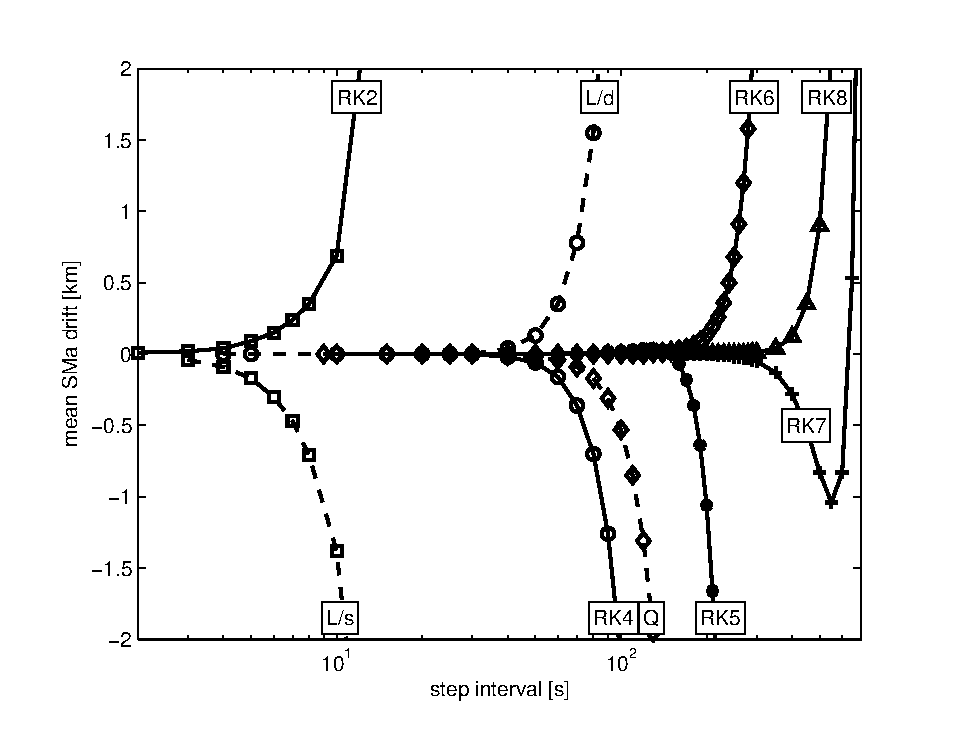
\includegraphics[width=0.99\textwidth]{sma_dev}\\
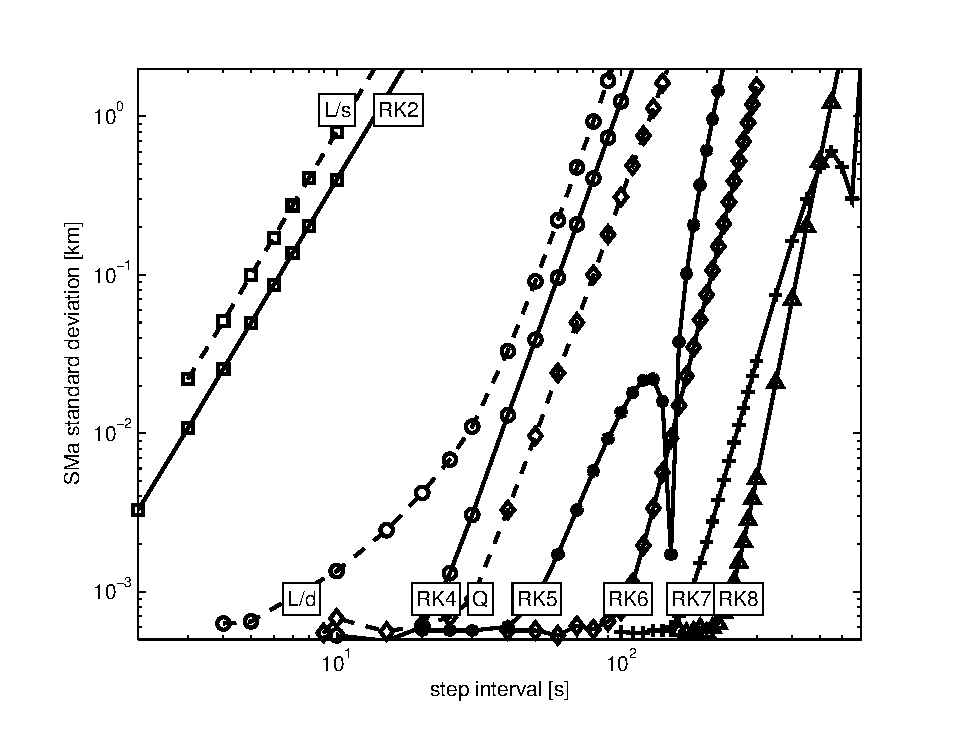
\includegraphics[width=0.99\textwidth]{sma_std}
\caption{Mean drift (top) and standard deviation (bottom) in semi-major axis for a low Earth orbit (mean altitude 217\,km) over a period of 10 days, as a function of time step length. Shown are the interpolation and Runge-Kutta families of integrators used in the Orbiter code.}
\label{fig:1day_err}
\end{figure}

\begin{figure}[H]\centering
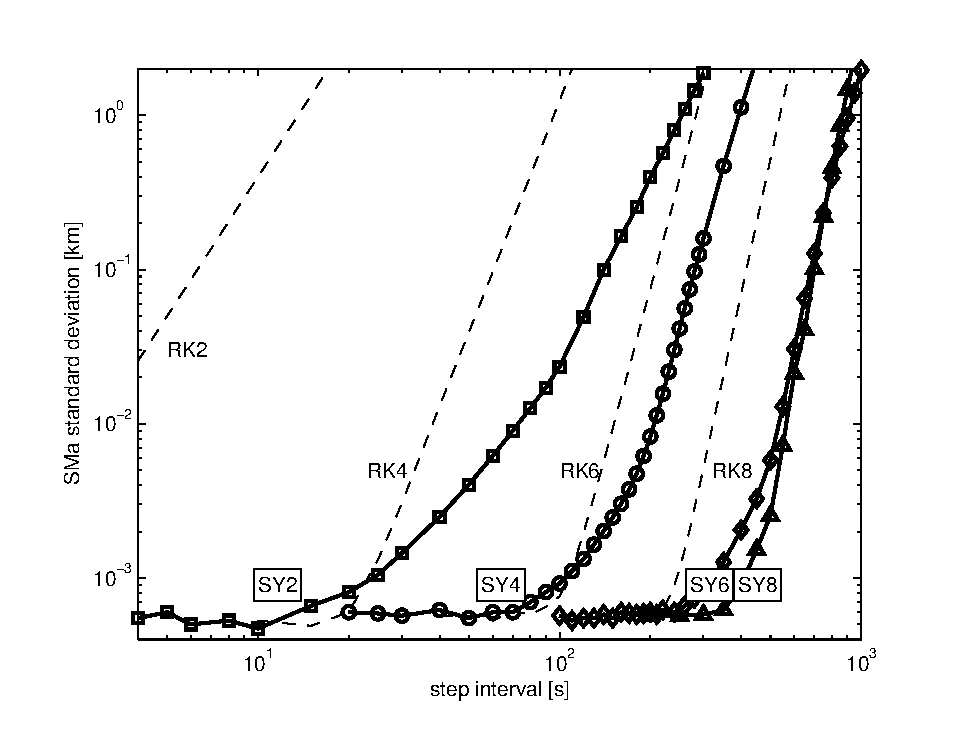
\includegraphics[width=0.99\textwidth]{sma_symp_std}
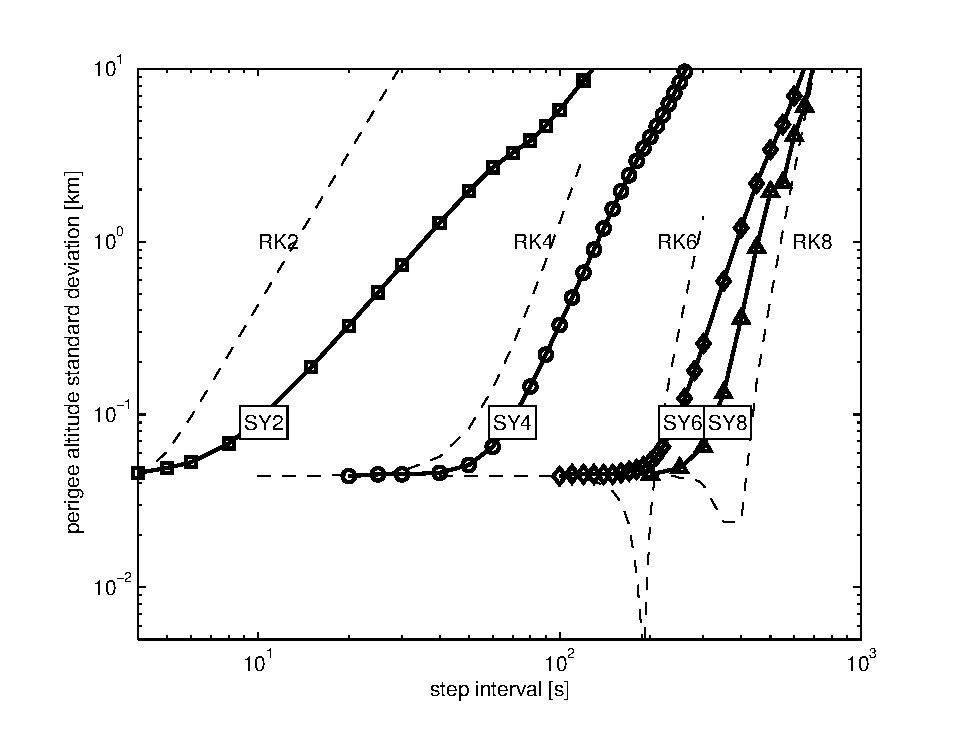
\includegraphics[width=0.99\textwidth]{pea_symp_std}
\caption{Standard deviation in semi-major axis (top) and perigee altitude (bottom) for the 2nd, 4th, 6th and 8th order symplectic integrators available in Orbiter. For comparison, the 2nd, 4th, 6th and 8th order Runge-Kutta results are shown as dashed lines.}
\label{fig:symp_err}
\end{figure}

Note that with default parameters, Orbiter will switch to ``stabilised'' orbit calculation for steps that involove a change in mean anomaly of more than $10^{-3} \cdot 2\pi$. In low Earth orbit with period $T\approx5400\,s$, this corresponds to a time interval of 5.4\,s.

For comparison, with a typical frame rate of 50\,fps and at a selected time compression of $1000\times$, the step interval is 20\,s. During normal simulation runs, the main problem are however isolated long steps, caused for example by disc I/O. During such steps, the orbit stabilisation mode keeps orbits from deteriorating. 

\end{document}
